\documentclass[10pt,a4paper]{article}
\usepackage[utf8]{inputenc}
\usepackage[T1]{fontenc}
\usepackage[provide=*,spanish]{babel}
\usepackage[margin=1.95cm,headheight=14pt]{geometry}
\usepackage{lmodern,microtype,amsmath,amssymb,booktabs,array,graphicx,xcolor,fancyhdr}
\usepackage[colorlinks=true,linkcolor=blue!45!black,urlcolor=blue!45!black]{hyperref}
\usepackage{enumitem}
\definecolor{azul}{HTML}{174A66}
\setlength{\parindent}{0pt}
\setlength{\parskip}{5pt}
\setlist{nosep,leftmargin=*}
\renewcommand{\arraystretch}{1.13}
\pagestyle{fancy}
\fancyhf{}
\fancyhead[L]{\small\color{azul}SIS210 · Algoritmos y Estructuras de Datos}
\fancyhead[R]{\small Semana 2}
\fancyfoot[L]{\small UNA Puno · Resultados del entorno remoto de Work}
\fancyfoot[R]{\thepage}
\newcommand{\titulo}[1]{\vspace{3pt}{\large\bfseries\color{azul}#1}\par}
\newcommand{\subtitulo}[1]{\vspace{2pt}{\bfseries\color{azul}#1}\par}
\newcommand{\referencia}[1]{\par\begingroup\small\setlength{\hangindent}{1.1em}\setlength{\parskip}{4pt}#1\par\endgroup}
\begin{document}
\hypersetup{pageanchor=false}
\begin{titlepage}
\centering
{\Large\bfseries UNIVERSIDAD NACIONAL DEL ALTIPLANO\par}
\vspace{0.25cm}
{\large Puno\par}
\vspace{0.7cm}
Facultad de Ingeniería Mecánica Eléctrica, Electrónica y Sistemas\par
Escuela Profesional de Ingeniería de Sistemas\par
\vspace{2.2cm}
{\color{azul}\rule{\textwidth}{1.2pt}}\par
\vspace{0.5cm}
{\Huge\bfseries\color{azul}Complejidad y búsquedas\par}
\vspace{0.5cm}
{\Large Comparación teórica y experimental\par}
{\large Búsqueda lineal y binaria en Python y C++20\par}
\vspace{0.5cm}
{\color{azul}\rule{\textwidth}{1.2pt}}\par
\vspace{1.5cm}
\begin{tabular}{rl}
\textbf{Curso:}&Algoritmos y Estructuras de Datos -- SIS210\\[6pt]
\textbf{Semana:}&2\\[6pt]
\textbf{Docente:}&ZANABRIA GALVEZ ALDO HERNAN
\end{tabular}
\vspace{1.1cm}
\par\textbf{Integrantes}\par
YANA MENDOZA CARLOS BENEDICTO\par
BELIZARIO YANA DAVID VICTOR\par
CURASI ZEVALLOS HANDDY RONALD\par
\vspace{0.8cm}
\textbf{Repositorio GitHub:}\par
\href{https://github.com/handdycurasi-crypto/SIS210-Semana02-Complejidad}{\texttt{github.com/handdycurasi-crypto/SIS210-Semana02-Complejidad}}\par
\vfill
{\large Puno -- Perú\par 2026\par}
\end{titlepage}
\setcounter{page}{1}
\hypersetup{pageanchor=true}
\titulo{1. Problema y objetivo}
Una colección de transacciones necesita localizar \texttt{CustomerID}. Se compara recorrerla directamente con buscar en una copia previamente ordenada. El objetivo es contrastar el crecimiento teórico con sondeos y tiempos reales, incluyendo el costo de preparar el orden. Se sigue la guía de Zanabria Gálvez (2026). Aunque su portada dice C++17 y Semana 1, las instrucciones operativas corresponden a C++20 y Semana 2; se adoptan estas últimas.

\titulo{2. Marco teórico: RAM, funciones de costo y cotas}
\textbf{Tamaño de entrada.} $n$ es el número de registros almacenados, incluidos identificadores repetidos; no es la cantidad de clientes distintos. El modelo RAM asigna costo constante a acceso, asignación, aritmética y comparación. Un conteo abstracto permite estudiar el crecimiento; no representa instrucciones exactas de CPU o bytecodes de Python.

\subtitulo{Derivación de la búsqueda lineal}
Se modela un recorrido equivalente al código: inicializar $n$, índice $i=0$ y contador $ops=0$; mientras $i<n$, examinar $a[i]$, incrementar $ops$, comparar con la clave y avanzar si no coincide. Cada operación cuesta 1; incrementar una variable cuesta 2 (suma y asignación). Se consideran obtener/asignar la longitud almacenada y retornar el par como operaciones abstractas unitarias. Se incluye la instrumentación.
\begin{center}\small
\begin{tabular}{p{8.4cm}rr}
\toprule
Operación & Ausente & Éxito en visita $k$\\\midrule
Inicializaciones de $n$, $i$ y $ops$ & 3 & 3\\
Control $i<n$ & $n+1$ & $k$\\
Acceso al elemento & $n$ & $k$\\
Incremento de $ops$: suma y asignación & $2n$ & $2k$\\
Comparación de igualdad & $n$ & $k$\\
Incremento de $i$: suma y asignación & $2n$ & $2(k-1)$\\
Retorno & 1 & 1\\\midrule
Total & $7n+5$ & $7k+2$\\\bottomrule
\end{tabular}\end{center}
Así, $T_{\rm ausente}(n)=3+(n+1)+n+2n+n+2n+1=7n+5$. Al inicio $k=1$, el costo es constante; al final $k=n$, es $7n+2$. El contador del CSV mide solo sondeos: $n$ en ausencia y $k$ en éxito. Cambiar el convenio RAM modifica constantes, no el crecimiento. Para $n\ge1$, $7n\le7n+5\le12n$: el peor caso es $\Theta(n)$.

\subtitulo{Cotas y casos son conceptos diferentes}
Para $n\ge n_0$, $O(g(n))$ exige $T(n)\le c g(n)$; $\Omega(g(n))$ exige $T(n)\ge c g(n)$; $\Theta(g(n))$ exige ambas con constantes positivas, posiblemente distintas. Se aplican a una función de costo ya definida. Por ejemplo, el peor caso lineal es también $\Omega(n)$ y su mejor caso también es $O(1)$. No se identifica $O$ con peor, $\Omega$ con mejor ni $\Theta$ con promedio (Cormen et al., 2022).

Con éxito, claves distintas y posiciones equiprobables, $E[ops]=(n+1)/2$ y el costo esperado lineal es $\Theta(n)$. Los duplicados y consultas no uniformes modifican esos supuestos. Repetir 30 veces una clave no estima el caso promedio probabilístico.

\subtitulo{Búsqueda binaria}
El orden permite descartar una mitad: $n\to n/2\to n/4\to\cdots$. Resolver $n/2^k\le1$ da $k\ge\log_2n$. Cada iteración hace trabajo constante: peor caso $\Theta(\log n)$ y mejor caso $\Theta(1)$ si coincide el primer centro. Con éxito uniforme y claves distintas, el promedio es $\Theta(\log n)$. La cota exacta de este código es $\lfloor\log_2n\rfloor+1$ sondeos para $n\ge1$; con $n=8$ puede hacer 4, precisando la aproximación de la guía. Ambas búsquedas iterativas usan $\Theta(1)$ memoria auxiliar, sin contar los datos.

\newpage
\titulo{3. Dataset y preparación}
Se descargó \textit{Online Retail} (Chen, 2015), DOI \href{https://doi.org/10.24432/C5BW33}{10.24432/C5BW33}, de UCI, bajo licencia CC BY 4.0. Se usó \texttt{CustomerID}, convertido a entero. El archivo observado contiene 541\,909 filas; se descartaron 135\,080 identificadores faltantes y quedaron 406\,829 registros válidos, con 4\,372 clientes distintos. Aunque la ficha web indica ausencia de faltantes, estos conteos proceden del Excel real. No se filtraron anulaciones, países ni importes: el problema es localizar claves, no estimar ventas.

Los 402\,457 registros adicionales respecto a clientes únicos se conservan; no equivalen necesariamente a filas completas duplicadas. Para cada $n$, la semilla es $21002+n$. Hasta 100\,000 se muestrean filas sin reemplazo. Para 500\,000 se remuestrean filas válidas con reemplazo: no se presentan como transacciones independientes adicionales.
\begin{center}
\begin{tabular}{rrrl}
\toprule
$n$ & Semilla & Clientes distintos & Muestreo de filas\\\midrule
100 & 21\,102 & 87 & Sin reemplazo\\
1\,000 & 22\,002 & 703 & Sin reemplazo\\
10\,000 & 31\,002 & 2\,667 & Sin reemplazo\\
100\,000 & 121\,002 & 4\,182 & Sin reemplazo\\
500\,000 & 521\,002 & 4\,344 & Con reemplazo\\\bottomrule
\end{tabular}\end{center}
\textbf{Escenarios exactos.} En cada muestra se seleccionan tres claves que aparecen una sola vez y se intercambian con las posiciones $0$, $n//2$ y $n-1$. Se conserva el multiconjunto y se garantiza primera coincidencia al inicio, centro y final. La clave ausente es máximo de la muestra más uno y no se agrega a los datos. Este condicionamiento permite contrastar casos; no representa la distribución de consultas de clientes reales.

Los CSV conservan \texttt{fila\_excel} y \texttt{CustomerID}. \texttt{metadatos.json} guarda limpieza, semillas y SHA-256 del origen y las muestras. Ambos lenguajes leen las mismas muestras y \texttt{claves.csv}. Lineal usa el orden preparado; binaria usa su copia ordenada. Los nombres de escenarios se refieren al orden original: el centro original no tiene por qué ser el centro de la copia ordenada.

\titulo{4. Diseño experimental}
La matriz tiene $5$ tamaños $\times\,2$ algoritmos $\times\,4$ escenarios $\times\,30$ repeticiones $\times\,2$ lenguajes: \textbf{2\,400 búsquedas individuales}. Hay un calentamiento por combinación y después se mezcla el orden de tareas con semilla $902+n$ en cada lenguaje. Las implementaciones se ejecutaron consecutivamente, no simultáneamente. Se conserva cada repetición y se calcula promedio, mediana, mínimo y máximo de tiempo y sondeos.

Python usa \texttt{perf\_counter\_ns()} y C++ \texttt{steady\_clock} con conversión a nanosegundos, conforme a su documentación (Python Software Foundation, s. f.; ISO/IEC JTC1/SC22/WG21, s. f.). Se cronometra la llamada instrumentada de búsqueda; carga, selección de función, copia, validación, ordenamiento e impresión quedan fuera. Ordenar se mide aparte, 30 veces por tamaño y lenguaje sobre una nueva copia: \textbf{300 ordenamientos}. La copia tampoco forma parte de ese tiempo.

\titulo{5. Implementaciones y control de variables}
Las búsquedas son manuales. Lineal retorna la primera coincidencia; binaria, una coincidencia de la copia ordenada. \texttt{comparaciones} conserva el convenio de la guía: un sondeo por elemento visitado. En binaria un sondeo puede ejecutar igualdad y menor-que; no es un conteo de todas las expresiones booleanas. Los resultados se verifican y se escriben fuera del intervalo; su uso observable evita tratar la búsqueda como cálculo sin efecto.

Se contrastaron 2\,070 consultas por lenguaje con oráculos de biblioteca, incluyendo vacíos, repetidos, negativos y límites. Se probó rechazo de desorden y errores de preparación. El análisis cruza claves, posiciones y sondeos entre lenguajes. La demo pequeña está separada del benchmark y permite ingresar una clave, elegir algoritmo, provocar desorden, corregir y repetir.

\textbf{Entorno real: Work remoto.} Linux 6.18.35 x86\_64; CPU visible AMD EPYC 9V74; memoria visible 16\,399\,700 kB, límite de contenedor 14 GiB; 9 CPU lógicas visibles y cuota equivalente a 8. Python 3.12.14, GCC 13.3.0; flags \texttt{-std=c++20 -O2 -Wall -Wextra -pedantic}. pandas 2.2.3, matplotlib 3.10.8 y openpyxl 3.1.5. No se atribuyen estas mediciones a la PC del estudiante.

\newpage
\titulo{6. Resultados teóricos y empíricos}
\subtitulo{6.1. Número de sondeos}
Los 80 grupos tienen 30 repeticiones. Python y C++ coinciden en posición y sondeos para cada consulta. La figura representa Python; la correspondiente de C++ está incluida y tiene los mismos conteos. Los ejes logarítmicos permiten visualizar desde un sondeo hasta 500\,000.
\begin{center}
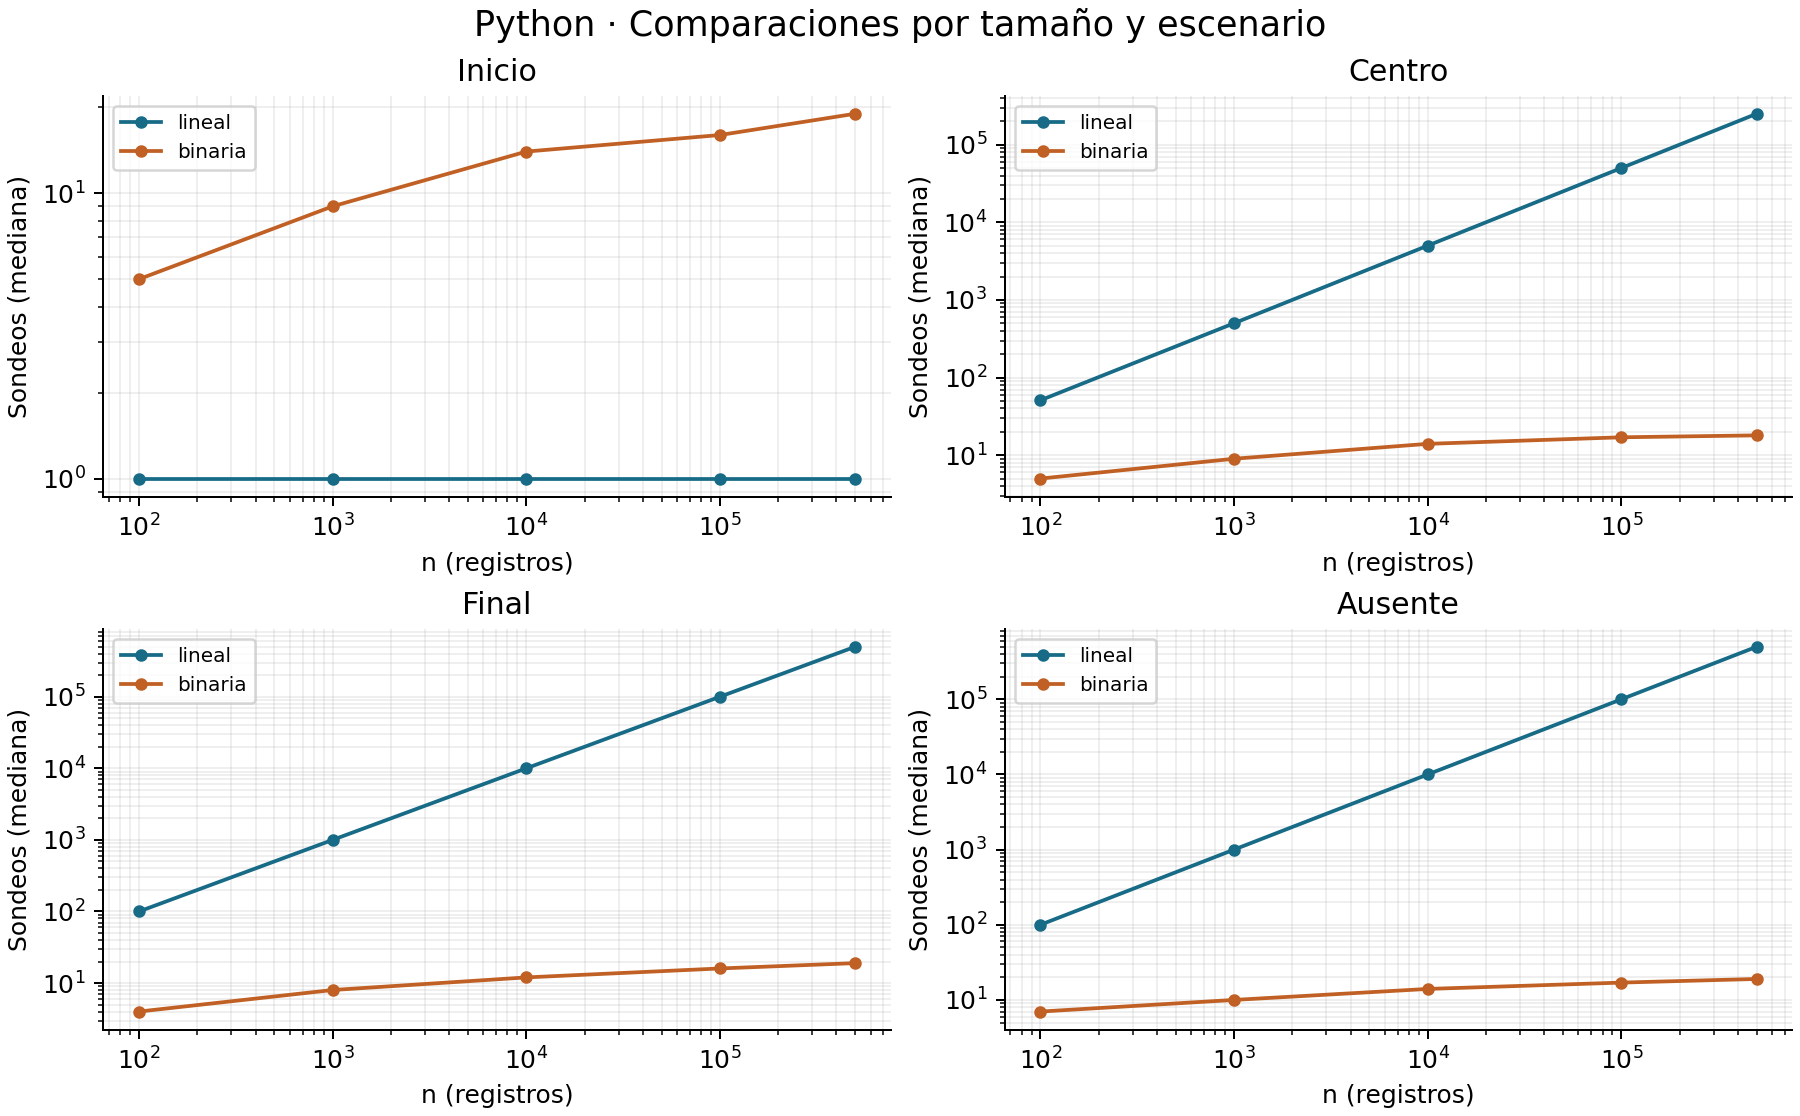
\includegraphics[width=\textwidth]{../graficos/comparaciones_python.png}
\end{center}
{\small\textbf{Figura 1.} Mediana de sondeos por tamaño y escenario. Fuente: ejecuciones reales de este proyecto. Inicio/centro/final designan posiciones en la muestra original.}

\begin{center}
\begin{tabular}{lrr}
\toprule
Escenario, $n=100\,000$ & Lineal & Binaria\\\midrule
Inicio & 1 & 16 \\
Centro & 50\,001 & 17 \\
Final & 100\,000 & 16 \\
Ausente & 100\,000 & 17 \\
\\[-6pt]\bottomrule
\end{tabular}\end{center}
{\small\textbf{Tabla 1.} Sondeos, iguales en ambos lenguajes. Las repeticiones no cambian este conteo determinista.}

El inicio lineal conserva un sondeo para todo $n$. El centro requiere $\lfloor n/2\rfloor+1$, el final requiere $n$ y la ausencia también $n$. Al aumentar de 100 a 500\,000, final y ausente crecen por un factor de 5\,000: se cumple la predicción lineal. La ausencia binaria pasa de 7 a 19 sondeos, consistente con el límite logarítmico.

Los casos exitosos de binaria no tienen que crecer monótonamente: cada muestra tiene claves y posiciones ordenadas diferentes. Lo que se contrasta es una cota, no una obligación de consumir exactamente $\log_2 n$ sondeos en cada consulta. Tampoco se espera que el centro original sea su mejor caso.

\subtitulo{6.2. Lectura de la evidencia}
El contador muestra crecimiento sin depender de la frecuencia del procesador. El reloj agrega información sobre constantes y entorno. Esta separación evita confundir escalabilidad con velocidad, distinción tratada por el repertorio de algoritmos del NIST (Black, 2020). La evidencia completa se conserva en \texttt{resultados\_crudos.csv} y \texttt{resumen\_estadistico.csv}; la tabla de esta página resume sondeos, no sustituye los estadísticos temporales.

\newpage
\subtitulo{6.3. Tiempos observados y costo de preparación}
\begin{center}
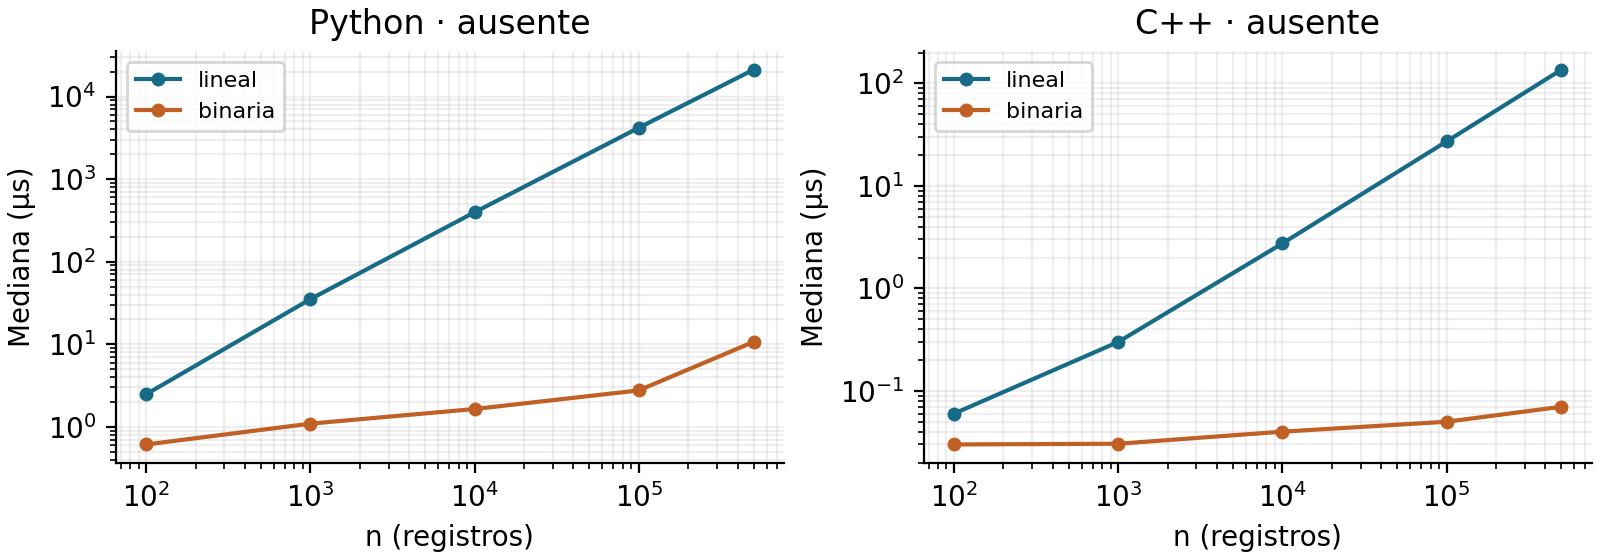
\includegraphics[width=\textwidth]{../graficos/tiempo_ausente.png}
\end{center}
{\small\textbf{Figura 2.} Tiempo mediano del caso ausente, por lenguaje, en microsegundos y ejes logarítmicos. Los cuatro escenarios de cada lenguaje se entregan en figuras separadas.}
\begin{center}\small
\begin{tabular}{llrr}
\toprule
Lenguaje & Escenario, $n=100\,000$ & Lineal ($\mu$s) & Binaria ($\mu$s)\\\midrule
Python & Inicio & 0.640 & 3.410 \\
Python & Centro & 2\,075.443 & 3.270 \\
Python & Final & 4\,185.722 & 2.969 \\
Python & Ausente & 4\,183.473 & 2.760 \\
C++ & Inicio & 0.030 & 0.050 \\
C++ & Centro & 13.590 & 0.055 \\
C++ & Final & 27.140 & 0.050 \\
C++ & Ausente & 27.140 & 0.050 \\
\\[-6pt]\bottomrule
\end{tabular}\end{center}
{\small\textbf{Tabla 2.} Medianas de 30 ejecuciones, redondeadas a 0.001 $\mu$s. El CSV conserva mayor precisión, promedio, mínimo y máximo.}

En ausencia con $n=500\,000$, las medianas son 21.106 ms y 10.676 $\mu$s en Python, frente a 135.952 $\mu$s y 0.070 $\mu$s en C++ (lineal y binaria, respectivamente). Son observaciones del código instrumentado en Work; especialmente los intervalos pequeños dependen del costo del reloj, caché y planificación del sistema.

\textbf{Una consulta frente a muchas.} Para datos estables, $C_L(q)=qL$ y $C_B(q)=S+qB$, donde $S$ es ordenar. Si $L>B$, binaria ofrece ventaja estricta cuando $q>S/(L-B)$. En ausencia con $n=500\,000$, $S$ mediano fue 73.373 ms en Python y 19.209 ms en C++. El primer entero favorable es $q=4$ y $q=142$, respectivamente.
\begin{center}\small
\begin{tabular}{lrrr}
\toprule
Lenguaje & $q$ & $qL$ (ms) & $S+qB$ (ms)\\\midrule
Python & 1 & 21.106 & 73.384 \\
Python & 1000 & 21\,105.963 & 84.049 \\
C++ & 1 & 0.136 & 19.209 \\
C++ & 1000 & 135.952 & 19.279 \\
\\[-6pt]\bottomrule
\end{tabular}\end{center}
{\small\textbf{Tabla 3.} Costos \emph{modelados} con medianas, para la misma consulta ausente y $n=500\,000$; no son lotes adicionales cronometrados. Se excluyen carga y copia.}

Para inicio lineal no hay amortización favorable en esta sesión porque $L\le B$. La conclusión depende de la consulta y del costo de mantener la colección: afirmar que binaria siempre gana sería incorrecto.

\newpage
\titulo{7. Discusión de discrepancias y limitaciones}
Los sondeos siguen la teoría, pero las medianas temporales no son funciones puras de $n$. El intérprete, la representación de enteros, la optimización del compilador, la localidad de acceso y la carga compartida alteran constantes. Se incluyó el contador y no se descontó el costo del reloj. Expresar un intervalo en nanosegundos no garantiza precisión física de un nanosegundo. No se fijó afinidad ni se aisló toda actividad del sistema.

Se usa una sola muestra por tamaño, 30 repeticiones de cada clave y calentamiento; por tanto no hay inferencia estadística sobre todas las transacciones o sobre consultas en frío. Las claves únicas elegidas condicionan deliberadamente los escenarios; los duplicados restantes se conservan y el tamaño 500\,000 usa reemplazo. El centro no estima por sí solo el caso promedio. Los estadísticos son descriptivos y no se construyeron intervalos de confianza.

La amortización supone costos por consulta estables y excluye copia, carga y actualizaciones. Una tabla hash podría ofrecer búsqueda esperada constante con memoria y colisiones; un árbol equilibrado ofrece búsqueda y actualización logarítmicas. Elegir una estructura requiere considerar el trabajo completo, no solo una llamada (Skiena, 2020). Los benchmarks y pruebas automatizadas se ejecutaron en el entorno remoto Linux/GCC de Work. La demo fue reproducida además en la PC del estudiante con Windows 10, Python 3.14.5 y MinGW GCC 14.2.0 incluido con Code::Blocks; se comprobó búsqueda lineal, búsqueda binaria y el rechazo de la búsqueda binaria cuando los datos están desordenados.

\titulo{8. Conclusiones}
\begin{enumerate}
\item La búsqueda lineal verifica costo constante al inicio y crecimiento lineal en centro, final y ausencia. Binaria respeta el límite logarítmico y necesita orden previo. Los conteos concuerdan en ambos lenguajes.
\item Las cotas $O$, $\Omega$ y $\Theta$ describen funciones de costo, mientras los casos describen entradas o distribuciones. Los tiempos observados no reemplazan la derivación RAM.
\item Ordenar puede compensar con suficientes consultas, pero no siempre con una sola ni para objetivos al inicio. Los umbrales calculados pertenecen a esta sesión y sus supuestos.
\item Los datos con procedencia, crudos, versiones, pruebas y comandos permiten repetir el experimento. La demo se reprodujo localmente en Windows y el repositorio se publicó con commits reales separados en \texttt{baseline}, \texttt{analysis}, \texttt{benchmark} y \texttt{final}.
\end{enumerate}

\titulo{9. Declaración de uso de IA}
Se utilizó ChatGPT para estructuración, apoyo de programación, revisión y documentación. Las implementaciones y los benchmarks se sometieron a pruebas y ejecución en Work; adicionalmente, las demos de Python y C++ fueron ejecutadas localmente en la PC del estudiante para verificar su funcionamiento y el manejo del requisito de ordenamiento. Los integrantes son responsables de revisar y comprender el trabajo antes de su sustentación.

\titulo{10. Referencias}
\referencia{Black, P. E. (2020). \textit{DADS: The on-line dictionary of algorithms and data structures} (NISTIR 8318). National Institute of Standards and Technology. \url{https://doi.org/10.6028/NIST.IR.8318}}
\referencia{Chen, D. (2015). \textit{Online Retail} [Conjunto de datos]. UCI Machine Learning Repository. \url{https://doi.org/10.24432/C5BW33}}
\referencia{Cormen, T. H., Leiserson, C. E., Rivest, R. L., \& Stein, C. (2022). \textit{Introduction to algorithms} (4.ª ed.). MIT Press. \url{https://mitpress.mit.edu/9780262046305/introduction-to-algorithms/}}
\referencia{ISO/IEC JTC1/SC22/WG21. (s. f.). \textit{Class steady\_clock [time.clock.steady]}. En \textit{C++ working draft}. Recuperado el 10 de septiembre de 2026, de \url{https://eel.is/c++draft/time.clock.steady}}
\referencia{Python Software Foundation. (s. f.). \textit{time -- Time access and conversions}. En \textit{Python documentation}. Recuperado el 10 de septiembre de 2026, de \url{https://docs.python.org/3/library/time.html}}
\referencia{Skiena, S. S. (2020). \textit{The algorithm design manual} (3.ª ed.). Springer. \url{https://doi.org/10.1007/978-3-030-54256-6}}
\referencia{Zanabria Gálvez, A. H. (2026). \textit{Guía de práctica de laboratorio: Semana 2. Algoritmos y Estructuras de Datos, SIS210} [Material de clase]. Universidad Nacional del Altiplano.}
\end{document}
